\RequirePackage{amsthm} %https://tex.stackexchange.com/questions/687324/unknown-theoremstyle-warning-with-springer-nature-template
\documentclass[sn-mathphys-num,iicol]{sn-jnl}

%\usepackage{sn-jnl.sty}
\usepackage{graphicx}%
\usepackage{multirow}%
\usepackage{amsmath,amssymb,amsfonts}%
\usepackage{amsthm}%
\usepackage{physics}
\usepackage[locale=DE]{siunitx}
\usepackage{mathrsfs}%
\usepackage[title]{appendix}%
\usepackage{xcolor}%
\usepackage{textcomp}%
\usepackage{manyfoot}%
\usepackage{booktabs}%
\usepackage{algorithm}%
\usepackage{algorithmicx}%
\usepackage{algpseudocode}%
\usepackage{listings}%
\usepackage{newtxmath}%
\usepackage{yfonts}
\usepackage{braket}
\usepackage{dsfont}
\usepackage[tiny]{titlesec}%
\usepackage[ngerman]{babel}

\theoremstyle{thmstyleone}
\newtheorem{theorem}{Theorem}
\newtheorem{proposition}[theorem]{Proposition}

\theoremstyle{thmstyletwo}
\newtheorem{remark}{Remark}

\theoremstyle{thmstylethree}
\newtheorem{definition}{Definition}

\raggedbottom

\newcommand{\td}{\text{d}}

\titleformat{\subsection}{}{\thesubsection}{1em}{\itshape}
\titleformat{\subsubsection}{}{\thesubsubsection}{1em}{\itshape}

\begin{document}
        
\title[]{Bestimmung des Quark-Antiquark Potentials in der Hamiltonischen Formulierung der kompakten U(1) Eichtheorie.}
\author*[1]{\fnm{Angelo} \sur{Brade}}\email{s72abrad@uni-bonn.de}
\affil*[1]{Rheinische Friedrich--Wilhelms--Universität, Bonn}

\maketitle
\newpage
\newpage
\section{}
\subsection{Discretisation}
We start by discretising the positional space into sites and links. The sites are spaced by the lattice spacing $a$. To optain the continuum theory in the limit of $a\rightarrow0$ we need to introduce the coupling constant $g$\cite{RevModPhys.51.659}.
\\
We associate each site with a corresponding positional vector $\vec{r}=(r_x, r_y)$. On the sites the static charges $Q_\vec{r}$ positioned. We associate each link with a corresponding position $\vec{r}$ and a direction $\mu$, where $-\mu$ is its opposite direction. For example with $\vec{r}=(1, 2)$ and $\mu=x$ we would denote the link that points from the site $(1, 2)$ to the $x$ direction. We could denote the same link with $\vec{r}=(2, 2)$ and $\mu=-x$.

On the links are the electric field operators $\hat{E}_{\vec{r},\mu}$ positioned. Each electric field $\hat{E}_{\vec{r}, \mu}$ has the vector potential $\hat{A}_{\vec{r}, \mu}$ as its canonical conjugate variable. Thus
\begin{align}
	[\hat{E}_{\vec{r_i}, \mu}, \hat{A}_{\vec{r_j}, \nu}]=i\delta^{(3)}(\vec{r_i}-\vec{r_j})\delta_{\mu\nu}.\label{eq:com}
\end{align}
We construct a unitary operator $\hat{U}_{\vec{r_j}, \nu}$ (also called link operator) by using the vector potential as the generator in the Lie algebra $\mathfrak{g}$. Thus through the exponential mapping we get the elements of the Lie group G:
\begin{align}
	\hat{U}_{\vec{r}, \mu} = e^{iag\hat{A}_{\vec{r}, \mu}}.\label{eq:exp}
\end{align}

The generated Lie group $G=\text{U}(n)$ has the complex matrix elements $\hat{U}_{\vec{r}, \nu}$ of dimension $n\cross n$. By taking $n=1$ we choose the U(1) theory, where the Phase, thus our vector potantial, is an element of $\mathbb{R}$. Through equation \ref{eq:com} and \ref{eq:exp} we arrive at
\begin{align}
	[\hat{E}_{\vec{r_i}, \mu}, \hat{U}_{\vec{r_j}, \nu}]      & =\delta^{(3)}(\vec{r_i}-\vec{r_j})\delta_{\mu\nu}\hat{U}_{\vec{r_j}, \nu},\label{eq:comu1}       \\
	[\hat{E}_{\vec{r_i}, \mu}, \hat{U}_{\vec{r_j}, \nu}^\dag] & =-\delta^{(3)}(\vec{r_i}-\vec{r_j})\delta_{\mu\nu}\hat{U}_{\vec{r_j}, \nu}\dag. \label{eq:comu2}
\end{align}

To explore the effect of the operators on the states, we choose to be in the electric basis with the basis states $\ket{e_{\vec{r_i}, \mu}}$. The basis is made up of all possible states at the links. We optain
\begin{align}
	\hat{E}_{\vec{r_i}, \mu}\ket{e_{\vec{r_i}, \mu}}=e_{\vec{r_i}, \mu}\ket{e_{\vec{r_i}, \mu}}.\label{eq:eig}
\end{align}
Furthermore with equation \ref{eq:comu1}, \ref{eq:comu2} and \ref{eq:eig} we get
\begin{align}
	\hat{U}_{\vec{r_i}, \mu}\ket{e_{\vec{r_i}, \mu}}      & =\ket{e_{\vec{r_i}, \mu}+1}\text{ and}\label{eq:eigu1} \\
	\hat{U}_{\vec{r_i}, \mu}^\dag\ket{e_{\vec{r_i}, \mu}} & =\ket{e_{\vec{r_i}, \mu}-1}.\label{eq:eigu2}
\end{align}
We see the unitary operators, also called linked operators, act as ladder operators.
\subsection{Truncation}
Since each field can be any real value, there are infinitly many possible fields for each link, thus constructing an infinitly dimensional basis. To be computable we truncate the possbile values, such that the basis is finite.

Revisiting the elements of U(1) we see, that they live on the unit circle in the complex plane. By limiting the phase of our exponential mapping in equation \ref{eq:exp} to $[-l, l]$, the phase is now an element of $\mathbb{Z}_{2l+1}$. This also truncates the electric field, such that $e_{\vec{r_i}, \mu}\in[-l, l]$. The unitary operators, which as we saw act as ladder operators to the eigenstates, can now also be expressed as
\begin{align*}
	\hat{U}_{\vec{r}, \mu} \mapsto \begin{bmatrix}
		                               0 & \,\dots\, & \,\dots \, & 0 \\
		                               1 & \dots     & \dots      & 0 \\
		                               0 & \ddots    & \vdots     & 0 \\
		                               0 & \dots     & 1          & 0 \\
	                               \end{bmatrix}, \hat{U}_{\vec{r}, \mu}^{\dag} \mapsto \begin{bmatrix}
		                                                                                    0 & 1          & \dots    & 0 \\
		                                                                                    0 & \vdots     & \ddots   & 0 \\
		                                                                                    0 & \dots      & \dots    & 1 \\
		                                                                                    0 & \,\dots \, & \dots \, & 0 \\
	                                                                                    \end{bmatrix}.
\end{align*}
The unitarity $\hat{U}_{\vec{r}, \mu}\hat{U}_{\vec{r}, \mu}^\dag\neq\mathds{1}$ for this is lot, but can be recovered in the continuum limit of $l\rightarrow\infty$. It is importend to point out, that we annihilate the first (last) state when using $\hat{U}_{\vec{r}}^{\dag}$ ($\hat{U}_{\vec{r}}$).
\subsection{Hamiltonian}
The Hamiltonian for the system was orgininally formulated by Kogut and Susskind \cite{PhysRevD.11.395} and thus since known as the so called Kogut Susskind Hamiltonian. It reads
\begin{align*}
	\hat{H}            = & \hat{H}_E+\hat{H}_B+\hat{H}_m+\hat{H}_{\text{kin}}\text{ with}                                                              \\
	\hat{H}_E          = & \frac{g^2}{2}\sum_{\vec{r}} \left(\hat{E}^2_{\vec{r},x}+\hat{E}^2_{\vec{r},y}\right),                                       \\
	\hat{H}_B          = & -\frac{1}{2a^2g^2}\sum_{\vec{r}} \left(\hat{P}_{\vec{r}}+\hat{P}^\dag_{\vec{r}}\right),                                     \\
	\hat{H}_m          = & m\sum_{\vec{r}}(-1)^{r_x+r_y}\hat{\phi}^{\dag}_{\vec{r}}\hat{\phi}_{\vec{r}}\text{ and}                                     \\
	\hat{H}_\text{kin} = & \frac{i}{2a}\sum_{\vec{r}}\left(\phi^{\dag}_{\vec{r}}\hat{U}_{\vec{r}, x}\phi_{\vec{r}+x}-\text{h.c.}\right)                \\
	                     & -\frac{(-1)^{r_x+r_y}}{2a}\sum_{\vec{r}}\left(\phi^{\dag}_{\vec{r}}\hat{U}_{\vec{r}, y}\phi_{\vec{r}+y}+\text{h.c.}\right).
\end{align*}

Firstly, lets get rid of the part we dont need. At the beginnen we introduced the static charges $Q_{\vec{r}}$. They are called static, since they cant move. We say that they have infinit mass, which implies they wont introduce any field and can not be moved. Thus the fermionic fields $\hat{\phi}_{\vec{r}}$ vanish at all $\vec{r}$. This premiss yields
\begin{align*}
	\hat{H}_{m}=\hat{H}_{\text{kin}}=0.
\end{align*}
The computation can also be done with dynamic charges $\hat{q}_{\vec{r}}$ where the mass and kinetik Hamiltonian will make contributions. In this case a phenomena called doubling problem will rise. A common approach for this problem are staggered fermions. We wont take a look at this and stay in the pure gauge case, where only gauge fields exist.

Now we take a look at the two remaining terms. The so called electric Hamiltonian $\hat{H}_E$ and the magnetic Hamiltonian $\hat{H}_B$. The latter originates from taking the real part of the plaquette operator $\hat{P}_{\vec{r}}$. It is the smallest Wilson loop (a closed loop through the lattice on the link operators) and the oriented product of the link operators, i.e.
\begin{align}
	\hat{P}_{\vec{r}}=\hat{U}_{\vec{r}, x}\hat{U}_{\vec{r}+x,y}\hat{U}^{\dag}_{\vec{r}+y,x}\hat{U}^{\dag}_{\vec{r},y},
\end{align}
where we denote e.g. $\vec{r}+x=(r_x+1,r_y)$. We take the hermitian conjugate of the two latter link operators since all link operators only show in positiv $x$ or $y$ direction and when going through the plaquette we are going against the orientation of the two last link operators. We see that by taking the hermitian conjugate of the plaquette operator, we just go through the plaquette the other way around.

The heuristic explaination of the form of the magnetic Hamiltonian is the following: The Plaquettes, as they are closed loops, are essentially conductor loops that introduce a magnetic moment by Farady's law, that is then measured by the magnetic hamiltonian. % TODO: is this correct?

Last but not least we take a look at the electric Hamiltonian. It is essentially the sum over each lattice site over the square of the electric field. Here we use the electric field operators $\hat{E}^2_{\vec{r},\mu}$. But not all of them are free. Gauss's law constraints about the half of them such that the others are truly free. The formulation reads
\begin{align}
	\left[\sum_{\mu=x,y}\left(\hat{E}_{\vec{r},\mu}-\hat{E}_{\vec{r}-\mu,\mu}\right)-\hat{q}_{\vec{r}}-Q_\vec{r}\right]\ket{\Psi}=0.
\end{align}
Here we sum over all electric field operators that are linked to a site $\vec{r}$ and are expecting them to be the same as the charge deposited on the site. Only those states $\ket{\Psi}$, which produce this relation, are thus physicaly possible. They live in the physical space $\cal{H}_{\text{ph}}$:
\begin{align}
	\ket{\Psi}\in\cal{H}_{\text{ph}},
\end{align}
where we denote by $\cal{H}$ the space in which a lattice configuration lives. Here the physical Hamiltonian is a subspace of the the complete Hamiltonian.

\subsection{Implementation}
For the implementation we construct the lattice and place all operators on thier place. Then we calculate each entry
\begin{align}
	\bra{i}\hat{H}\ket{j}.
\end{align}



\begin{figure}[h]
  \begin{center}
    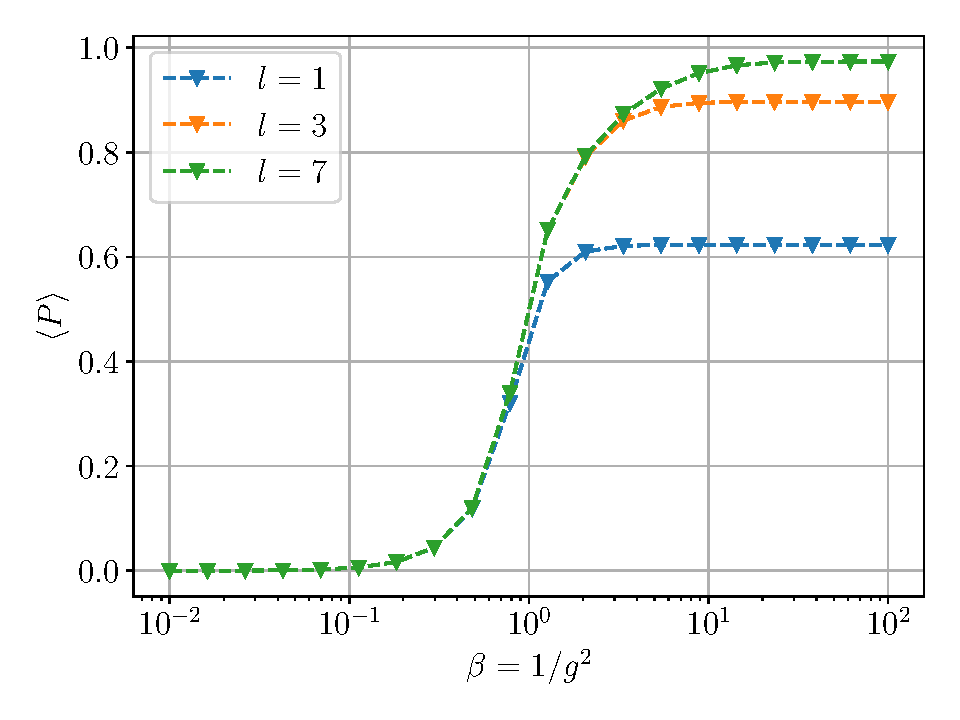
\includegraphics[width=0.45\textwidth]{images/PlaquetteExp2x2PBC.pdf}
  \end{center}
  \caption{Plaquette expectation values for 2x2 pbc lattice.}
\end{figure}

%\input{sections/plaqueteexp.tex}

\bibliography{refs}
\end{document}
